\chapter{System Description}\label{chap:sys_description}
The present chapter covers the system design including specific solutions that have been chosen for the realization of the SmartNotes application. The system concept, introduced in Chapter~\ref{chap:concept}, will become extended by describing certain elements of implementation and problems found during the development process. This should allow the reader to have a deeper view into the SmartNotes application, including the functions that it offers as well as the platform that it runs on.
\section{Google App Engine platform}\label{sec:gae}
Google App Engine seems to be an outstanding development platform. For all the reasons mentioned in~\ref{sec:gae_general}, it has been decided to be used as the main platform for SmartNotes as the one preceding any other hosting services. Besides, GAE appears to be highly competitive in terms of cost calculations, which are described in Section~\ref{subsec:gae_calculations}. After registering the application with a unique name, it can be easily uploaded to Google and after a few seconds it is accessible to its users.

As stressed in Section~\ref{subsec:sync_scenarios}, synchronization scenarios use the client-server architecture. When running on GAE platform which is, as mentioned in~\ref{sec:gae_general}, a distributed vault-tolerant infrastructure where two subsequent request may be served by different machines located in separate data centres. Thus in the addressing scope, the application can still be treated as a centralized server. In case the application requires state awareness, it is the developer's role to make it so. Otherwise, the fact that the application is served from multiple machines is completely transparent from the functional point of view.

SmartNotes uses only some of the components supported by GAE and the ones which make a part of the SmartNotes application with relation with other third-party elements are presented in Figure~\ref{fig:smartnotes_components}. This is especially important as it presents all the application top level components together with marked interfaces between the particular functional blocks. This particular diagram strongly corresponds with the diagram from Figure~\ref{fig:ismartnotes_smartnotes}, which in a more general way presents the cooperation of SmartNotes and iSmartNotes with differentiated roles of the administrator and the user. 

The most complicated structure is the SmartNotes component, which is marked as an individual system. It does not require the iSmartNotes to realize its functionality. For this reason, the SmartNotes component could work with any kind of client application using the interface that the tool provides, or the interface of Mercurial HTTP chains of requests and responses that needed a back-end redesign to accommodate conditions set by GAE. The issues connected with the cooperation of Mercurial and GAE are the topic of Section~\ref{sec:hg_on_gae}. 

Furthermore, SmartNotes uses three additional interfaces which are used to interconnect the Google App Engine component with Mercurial adopted to run on GAE as well as separately, admin and user interfaces provided by SmartNotes. Each of the three components is connected in a different way. Whereas the webapp framework has a low Python overhead as mentioned in Section~\ref{subsec:webapp} and was chosen to serve the connection between the Mercurial and the Google App Engine componet, for performance reasons, it is Django which is the best choice when it comes to building nontrivial web-based functionality for reasons mentioned in Section~\ref{subsec:django}. The remaining two elements used by the GAE subsystem are the Google Account and the Datastore. The role of the first one has been presented in detail while discussing the iSmartNotes activation process in Section~\ref{subsec:ismartnotes_activation}. Some of the Datastore details will be covered in Section~\ref{sec:hg_on_gae}. 
\begin{figure}[ht]
\begin{center}
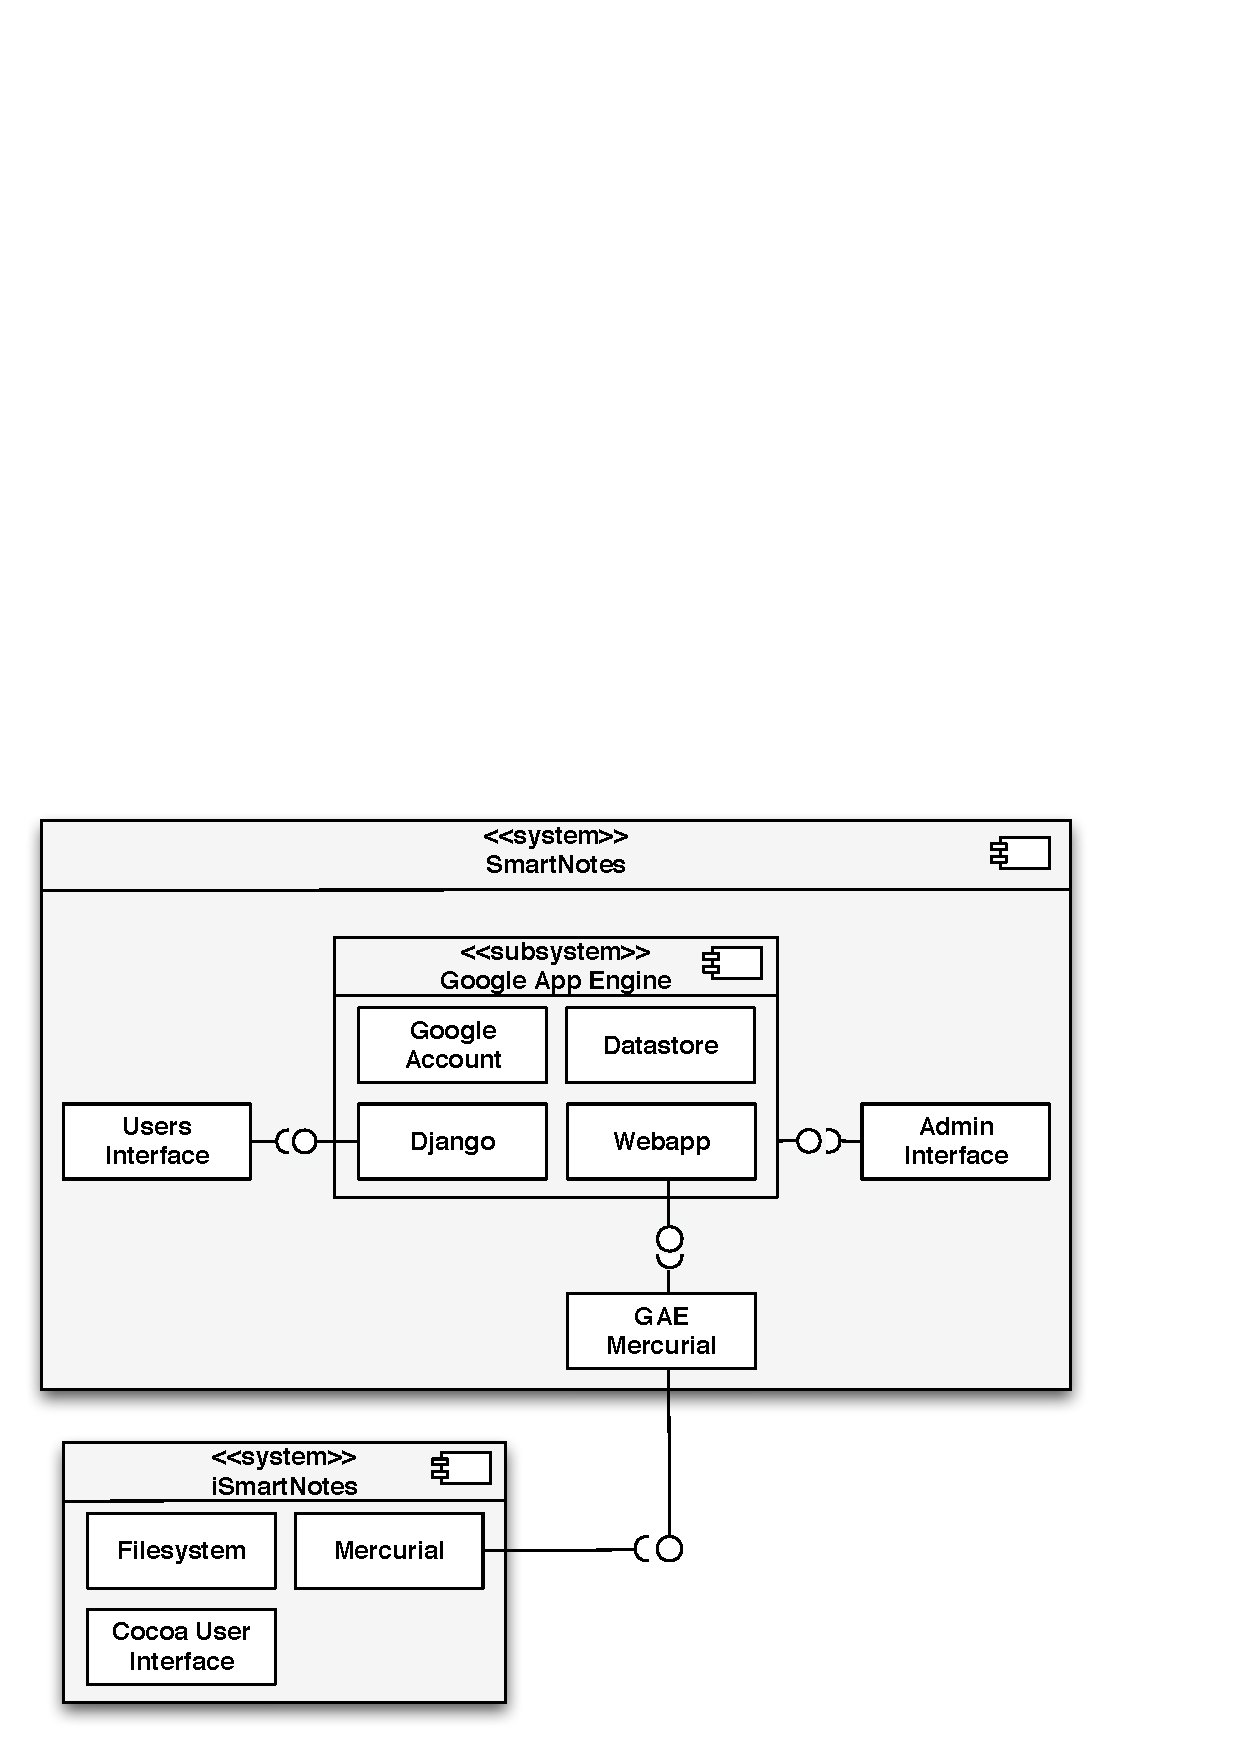
\includegraphics[scale=0.6]{charts/smartnotes_componets.png}
\caption{The components diagram of the SmartNotes application with marked interfaces between the functional blocks.}
\label{fig:smartnotes_components}
\end{center}
\end{figure}

The second independent system is the iSmartNotes component, which remains independent until the user decides to activate it to use the synchronization feature. For this purpose, it requires a Mercurial server to interact with. The iSmartNotes, as presented in Figure~\ref{fig:smartnotes_components}, is build with three components. Firstly, the file system of the client's operating system which is the classical space where VCS's allocate their repositories. Secondly, Mercurial VCS which on the client site does not require any modifications. Finally, the Cocoa user interface which is  discussed in Section~\ref{sec:cocoa}.

\subsection{Financial calculations}\label{subsec:gae_calculations}
The role of this section is to introduce some basic calculations that should give the reader a general experience of what kind of resources will be used by the application with the connection to the billing rates set by Google. In the next step this values will be used to predict the order of size for monthly cost of running the application for  one million of SmartNotes users. This should should help to indicate the system elements that generate highest price of resource usage what in the end lets to concentrate on optimization in those specific area. 

Calculations bellow aim to predict theoretical monthly cost of running SmartNotes applications for one million of users with unit price detailed in Table~\ref{tab:gae_cost}. Each of resources will become briefly introduced with short explanation of taken assumptions. The outcome of this considerations is illustrated in Figure~\ref{tab:gae_cost}.
\begin{table}[h]
\centering
\caption{Google App Engine billing rates on September 2009.}
\label{tab:gae_cost}
\begin{tabular}{|l|l|l|} \hline \hline
\textbf{Resource} & \textbf{Unit} & \textbf{Unit cost} \\ \hline \hline
Outgoing Bandwidth & Gigabytes & \$0.12 \\ \hline
Incoming Bandwidth & Gigabytes & \$0.10 \\ \hline
CPU Time & CPU hours & \$0.10 \\ \hline
Stored Data & Gigabytes per Day & \$0.005 \\ \hline
Recipients Emailed & Recipients & \$0.0001\\ \hline \hline
\end{tabular}
\end{table}

Resource usage to price calculations:
\begin{itemize}
\item{\textbf{Outgoing Bandwidth}. This value represents a summarized amount of data send from the server to the users. That normally includes html, css, java script and graphic files as the standard web pages components. In classical case a total size of a web page is round \mbox{70--150KB} what with compression can reduce it by factor of about 40\%. In case of SmartNotes application the content sent between the server and iSmartNotes are the changesets. It was assumed that the size of average downstream changeset won't exceed 2KB. It is smaller from the upstream changeset as not all server responses contain a changeset. A changset is sent only if there is a need for it what happens when there application encounters differences requiring to be synchronized.   

Next made assumption regards the users activity. As stated in the beginning the calculations are done for one million of users. Additionally among this users there is a strong group of active users what translated into numbers would mean that about 80\% of users generate four editing actions. This accordingly to the synchronization scenario from Figure~\ref{fig:seq_commit} might require sending the data from and to the server.  For this reason the the bandwidth calculations for incoming and outgoing traffic use the same number of requests. This all leads to the fallowing numbers:

$Outgoing\ Bandwidth =  80\% \cdot 1,000,000\ users \cdot 4\ requests\ per\ user \cdot$\\ \hspace*{37mm} $2KB\ per\ request \cdot 30\ days \approx \textbf{183GB\ per\ month}$ \\ 
$Outgoing\ Bandwidth\ Cost = 183GB\ per\ month \cdot \$0.12\ per\ GB \approx \textbf{\$22 per\ month}$ }

\item{\textbf{Incoming Bandwidth}. In this case the same number of requests will be used just as in case of outgoing bandwidth. That is 3,200,000 of requests per day and it will be used as basic parameter in all of undermentioned calculations. 

The size of a single request will be double the value taken when calculating the outgoing bandwidth. This is cause each of the operations done by use of iSmartNotes requires sending a changeset. Remaining part of calculations regarding incoming bandwidth follows the numbers which were used for outgoing bandwidth:

$Incoming\ Bandwidth =  3,200,000\ requests\ per\ day \cdot 4KB\ per\ request \cdot 30\ days$\\ \hspace*{33mm} $\approx \textbf{366GB\ per\ month}$ \\ 
$Incoming\ Bandwidth\ Cost = 366GB\ per\ month \cdot \$0.1\ per\ GB \approx \textbf{\$37 per\ month}$ }

\item{\textbf{CPU Time}. This calculation was done by checking the average time that the CPU was idle during serving a single request. As mentioned in Section~\ref{subsec:webapp} has lower Python overhead and for performance reasons it was chosen over the Django framework. This in consequence allowed to reduce the CPU time parameter. Due to the fact that all requests require CPU time the base number of 3,200,000 requests per day is multiplied by two for upstream and downstream requests. Turning that into numbers gives:

$CPU\ Time =  3,200,000\ requests\ per\ day \cdot 2 \cdot 0.02\ seconds\ per\ request \cdot 30\ days$\\ \hspace*{17mm} $\approx \textbf{1067\ hours\ per\ month}$ \\ 
$CPU\ Time\ Cost = 1067\ hours\ per\ month \cdot \$0.1\ per\ hour \approx \textbf{\$107 per\ month}$}

\item{\textbf{Stored Data}. To help imagine the storage space needed for an average notes repository let say that the popular collection of stories called "Winnie-the-Pooh" contains about 4,000 lines and it size in plain text without graphics is about 150KB. When using Version Control Systems it should be remembered as it was mentioned in Section~\ref{subsec:hg} that this systems consume additional disk space. The fudge factor saying how may times the final repository  size will be greater from the its base content size is about 3--4 times. That depends on how many files are stored in that repository and how frequent the changes are. Altogether assuming a size of 1MB for user repository seems to be reasonable and will make the calculations simple.

$Stored\ Data =  1,000,000\ users\cdot 1MB\ per user \cdot 1\ month \approx \textbf{977GB\ per\ month}$ \\ 
$Stored\ Data\ Cost = 977GB\ per\ month \cdot \$0.15\ per\ GB\ per\ month \approx \textbf{\$146 per\ month}$}

\item{\textbf{Mail}. In case of iSmartNotes activation there is no need to send mails to users like in a case of classical account creation what was discussed in Section~\ref{subsec:ismartnotes_activation}.On the other hand mail remains a very effective way to communicate with users. Although they are other possibilities like twitter\footnote{Twitter is an micro-blogging application allowing to share ideas and live-stream informations in the macro scale by the use of Internet.}, placing information on a web page or displaying dialog windows from the application, mailing users with the information remains more solid and professional attempt. For that reason it seems to be worth to take mailing service into account for keeping the users updated just as for sending invitations to potential new users. The additional 20\% of mails send is reserved just for that purpose --- allowing satisfied users to share the information about SmartNotes with their contacts.

$Mail =  1,000,000\ users\cdot (1 + 20\%) = \textbf{1,200,000\ mails\ per\ month}$ \\ 
$Mail\ Cost = 1,200,000\ mails\ per\ month \cdot \$0.0001\ per\ mail = \textbf{\$120 per\ month}$}
\end{itemize} 

This all together encloses in about \$312 without mailing and about \$432 with mailing service. Beside this the application may use the free quota up to limits which are shown in Table~\ref{tab:gae_free}. The free quota resources should allow to reach a rate of 5 million page views per month what could be used to serve the SmartNotes  homepage or as some backup resources for the application. 
\begin{table}[h]
\centering
\caption{Google App Engine free quota limitations on September 2009.}
\label{tab:gae_free}
\begin{tabular}{|l|l|} \hline \hline
\textbf{Resource} & \textbf{Daily Limit} \\ \hline \hline
Outgoing Bandwidth & 1 Gigabyte \\ \hline
Incoming Bandwidth & 1 Gigabyte \\ \hline
CPU Time & 6.5 CPU hours \\ \hline
Stored Data & 1 Gigabyte \\ \hline
Recipients Emailed & 2000 \\ \hline \hline
\end{tabular}
\end{table}

Prior calculated figures could be compared to some popular hosting services like Rackspace or Amazon Web Services that offer same resources for prices that are gathered in Table~\ref{tab:services_price_compare} . 
Some services like Joyent or Rackspace are were using some other pricing strategy by using base service price with predefined resources and allowing user to extend it by ordering additional resources. Because of this it is hard to make objectively compare resources prices in separate thus more accurate is to concentrate on the vales presented in Table~\ref{tab:services_price_compare} \emph{Summary} rows.    

Disregarding pricing differences it should be stressed that Google App Engine is not only a hosting service but also exposes for wide use Google infrastructure components that were mentioned in Section~\ref{sec:gae_general} . Furthermore developers which decide to use Google App Engine get access to a bunch of useful API's such as Memcache or URLfetch. Finally the dashboard not only gives a clear view on the application status but also lets to flexibly control the expanses. It allows to set a daily budget that might be changed anytime during the day. When some capital becomes unused it will be available in the next days. On the other hand applications using Google App Engine are protected  from running out of resources by load peaks\footnote{This effect is has a popular name, it is said that application become \emph{slashdoted} what might be the result of placing link to an application on some highly popular social web services like \url{slashdot.org} from which the effect takes name or becoming a target of malicious scripts or load testing programs.}. For all those reasons Google App Engine seems to be not only the most developer friendly and flexible platform but also offering a highly competitive pricing policy.   

\begin{table}[h]
\centering
\caption{SmartNotes resource prices among different hosting providers.}
\caption*{ $^{*}$ This prices couldn't be listed as some services use predefined resource sets and allow to bay extra resources.\\
 $^{**}$ This prices were calculated by using extra bandwidth and CPU time as mailing is not separately billed by those services. That was done by taking following constants: $Average\ Mail\ Size = 100KB$, $CPU\ Time\ per\ 100\ Mails = 0.01s$\\
 $^{***}$ This prices does mot include mail service as it is supplementary for SmartNotes application.}
\label{tab:services_price_compare}
\begin{tabular}{|l|l|l|l|l|} \cline{3-5}
		  \multicolumn{2}{c|}{}       &\multicolumn{3}{c|}{\textbf{Resource Price by Service}} \\ \hline \hline
\textbf{Resource} &\textbf{Quantity} &\textbf{Google}        &\textbf{Amazon}         &\textbf{Rackspace} \\ 
			     &			   &\textbf{App Engine} &\textbf{Web Services} &  \\ \hline \hline
Bandwidth &550 Gigabytes &\textbf{\$59} &\$68 &\$69 \\ \hline
CPU Time &1067 Hours &\$107 &\$170 &\textbf{\$48}\\ \hline
Stored Data &977 Gigabytes &\$146 & \$216 &\$146 \\ \hline
Mail &1,200,000 Mails &\$120 &\textbf{\$20}$^{**}$ &\$26$^{**}$ \\ \hline \hline
\multicolumn{2}{|c|}{\textbf{Summary}} &\$432 &\$474 &\$100$^{*}$+\$289=\textbf{\$389}\\ 
\multicolumn{2}{|c|}{} &\textbf{\$312}$^{***}$ &\$454$^{***}$ &\$100+\$263=\$363$^{***}$\\ \hline \hline
\end{tabular}
\end{table}

Presented bellow charts in Figure~\ref{fig:gae_cost} can be used to indicate the resources that usage costs most. From the visualized proportion it is clear that bandwidth is not that an issue as storage, mailing or the CPU time. When mailing service as mentioned before remains supplementary by making some optimization on storage the price could become reduced. One of possible ways is to reduce the history size that is stored with the notes repository. By creating a queue task\footnote{This is one of the Google App Engine features that was introduced in Section~\ref{sec:gae_general} that allows to run tasks in background when the system is not busy.} that would reorganize the SmartNote repositories to store only 20 most recent changsets the repository size might get reduced up to 50\%.      

\begin{figure}[ht]
  \begin{center}
    \subfigure[\textbf{Without mailing service}.]{\label{fig:gae_cost_without_mail}\includegraphics[scale=0.45]{img/price_div.png}}
    \subfigure[\textbf{With mailing service}.]{\label{fig:gae_cost_with_mail}\includegraphics[scale=0.45]{img/price_div_mail.png}}
  \end{center}
  \caption{Simulated monthly cost division of resources expected to be used by one million of SmartNotes users on Google App Engine.}
  \label{fig:gae_cost}
\end{figure}

\subsection{Scalability}
Scalability was one of the main design concerns by concerns of the presented project. SmartNotes application as mentioned in Chapter~\ref{sec:Introduction} was mend to meet scalability requirements same as care for the best user experience. Additionally the architecture should allow for future development flexibility. In classical case the applications can scale up to some relatively low level. Successfully implementing scalability patterns allows to shift this point further in the by keeping the cost growth linear depend on served traffic.  

Identifying SmartNotes  scalability barriers was the first essential step in the planning phase. Next some possible solutions were considered that  finally allowed to take architectural decisions and start the work on implementing them.   
\begin{itemize}
\item{Data retrieval. This superficially trivial problem becomes a true bottleneck for many systems aggregating data. In most popular case time needed to get some certain data from database is proportional to number of stored data. Scalable data retrieval model implies to make the time needed to find and return data proportional to the amount of queried data disregarding the number of data stored in database. Besides increased system load should have a minimum effect on system performance. This requires using a well prepared architecture and allowing for flexible memory administration. All of this is requirements are met by BigTable and are extremely hard to achieve when classical relational database  is used. This systems are of great use when there stored data does not have the potential of dramatical growth or can be easy become partitioned but can have a big impact on development process.  

In case of SmartNotes the data is organized in structures defined by Mercurial version control system. They should become organized that way that access to this structures should be optimal in a scope of particular user. That is especially a matter when the data is stored on multiple machines that can be possibly located in distant data centers. Minimizing this interoperation's or or ensuring constant duration is a serious scalability concern. As it was prior identified by Google engineers a production ready solution is available. Placing related entities in structures called entity groups causes them to be stored close on the disk space what results in less varied access time. By eliminating the fluctuations the data retrieval might deliver same level of latency disregarding total amount of stored data.}
\item{Bandwidth. This parameter may become crucial when the application bandwidth usage is significant. Once because it will cost money twice because the maximum allowed link throughput might reached. This considered together with network latency fluctuations motivate minimizing the size and number of transfered packages.

Effective usage of HTTP protocol was important concern by choosing a Version Control System. Mercurial characteristics~\cite{google_hg_git_compare} were one of it greatest advantages. Basing on it SmartNotes may form better bandwidth utilization by varying the synchronizing changesets rate. Because base configuration was satisfied the limitations set by Google none additional optimization techniques was used. One execution is the synchronization feature which was discussed in Section~\ref{subsec:sync_scenarios} while presenting synchronization scenarios on Figures~\ref{fig:seq_commit} and \ref{fig:seq_commit2}. On the other hand it is important to clearly note that this issue is one of the system fundaments and deserves close attention during further development.}
\item{Framework. Referring to the notes made in Section~\ref{sec:scalability} regarding the scalability therm it is not any particular technology that makes the application scale well. Neither it is easy to form general best practices for building web applications nor a one hundred guarantee recipe exists. Scalability becomes a part of application planing therefore depends strongly on the application characteristics. In effect of successfully implemented scalability patterns the final result might be a \textit{"system that dosn't need to change when the size of the problem changes"}\cite{mike_malone_quote}. 

For all of those aspects mentioned framework choice is not the most crucial decision. On the other hand well structured framework can play a very important role in the development cycle. Once it provides a frame for the application where the developer complements the parts that the application will use and twice it often ships with functional blocks that are ready to be used in the application. Adding a clear structure and great documentation is what makes the main decision criteria. In case of SmartNotes it was important to serve Mercurial synchronization feature by a minimum Python overhead framework that would allow for extensive HTTP protocol control. Rest of offered functionality should be realized by elastic framework that allows for rapid prototyping and that would care for the way the project is organized. This motivates the frameworks choice from Figure~\ref{fig:smartnotes_components}. This is what appeared to be the best choice for Python with combine with Google App Engine platform.    
}   
\end{itemize}
\subsection{Security considerations}\label{subsec:security}
Security just like scalability are topics of great importance especially for application that  are mend to be exposed for broad usage. Having that in mind the fallowing section aims to make the reader familiar with main attempts used to secure the SmartNotes application. The weakest points of network applications are all kind of interfaces that that they exposes to the users or client applications.  Therefore security issues raised in this section will regard the components interfaces  that were presented in Figure~\ref{fig:smartnotes_components}. The list of those security patterns fallows:
\begin{itemize}
\item{SSL for all authenticated requests. By using this common technique all the private data will be exchanged between user and server using the encrypted connection. Therefore event access to the network traffic records wont allow for taking over credentials or any of private data from SmartNotes users. 

This kind of protection has become a very standard and probably therefore Google decided to support it yet in the main configuration file. The basic form of \texttt{app.yaml} contains two sections. When the first one defies the application top level parameters like version, runtime or application identifier the role role of second is make URL dispatching by defining regular expressions witch actions that should become performed when a incoming URL matches a particular regular expression. One option supported options is done by key \texttt{secure} that is used with combination with one of three valid values \texttt{always}, \texttt{never} and \texttt{optional}. This parameter decides whether the request should become redirected to HTTP or HTTPS in case of secure connection.}

\item{Secure Authentication. This element has often a key value for security of entire system. The way authentication parameters are created and restored is what should be measured in two scales. First it should be designed with he the user in mind as by requiring two different and secure passwords the system will gain on security but may discourage lots of potential users. Secondible application designers should treat seriously security aspects and be able to find a middle ground between the reasonable level of security and user friendliness.

Because Google is a huge international company with constantly increasing number of products that gather new users it treats security aspects with a high priority. The Google account management allows to access multiple services simultaneously with the use of a single account. This makes it easy for users to try out Google new services and increases the increases the importance of the authentication. A malicious application that would gain the Google account credentials would give its author the right to access all of the Google services using stolen identity. This includes not only read access but also full write privileges allowing to modify or even delete its victim data. Google being aware of this threat made the authentication system well protected against all kind of intruders.

When considering a authentication system for SmartNotes it seemed that Google account is a best choice for authentication service. Google has proven that users can relay on their products and additionally in case of authentication it is a part that Google depends oneself. That makes it future save and additionally easy lets to be integrated in the application logic. This includes webapp just as the Django framework. Lets assume that the dashboard functionality requires prior authentication. In that case the part of configuration file could look as fallows: 
\lstset{language=Python,caption=Part of SmartNotes application configuration file app.yaml.,label=code:app_yaml_secure,
basicstyle=\scriptsize,         % the size of the fonts that are used for the code
showspaces=false,               % show spaces adding particular underscores
showstringspaces=false,         % underline spaces within strings
showtabs=false,                 % show tabs within strings adding particular underscores
tabsize=2,                    % sets default tabsize to 2 spaces
captionpos=b,                   % sets the caption-position to bottom
breaklines=true,                % sets automatic line breaking
breakatwhitespace=false,        % sets if automatic breaks should only happen at whitespace
escapeinside={\%*}{*)}          % if you want to add a comment within your code
}
\lstinputlisting{src/samples/app_yaml_secure.yaml}
Here as it was mentioned in previous point by use of a regular expression developer can define action with additional parameters to be used to served a particular group of requests. In this case urls \url{/dashboard/}, \url{/en/dashboard/} or \url{/es/dashboard/get_activation_key/} match the url pattern from Listing~\ref{code:app_yaml_secure} and will become served by \texttt{main.py} script. When the the dispatcher becomes queried with one of this urls it will first check whether user is authenticated if so it will serve the request using HTTPS otherwise the user will become redirected to a standard Google account login page and after successfully passing username and password will become redirected back to the dashboard.}
\item{Protecting user identity. All described before patterns protect help to fulfill that role. This point addresses this problem but from some slightly different view. This relates to two problems that needed to become solved to realize the SmartNotes functionality.

First one regards usage of user identifier for making personalized requests.This technique is used to uses to minimize data stored in session and session queries. However using a plain user identifier in the url is a serious security danger. Any logged in usser may try his luck to check what happens when he changes for i.e. \texttt{userid} parameter in the browser url bar. With couple of tries his curiosity could become rewarded in uncontrolled access to some other user data. That is also a good example for the these that security remains a developer responsibility and that he should not base on the security claims of tools he uses. When choosing this technique the user identifier should be protected by some hashing function with salt. That way it fairly harder to guess somebody's else identifier. However it still possible and to be sure that user that wants to use some identity should have a cookie with set from that domain with some random value. But this is amount exactly the definition of how session mechanism work. For that reason the best solution is to us e session to authorize requests. Thus SmartNotes uses session for authenticating and building personalized web pages.    

Second problem arises with the will of making a SmartNotes interface that would work from outside the web browser. This requires also user authentication and probably using setting some of user specific settings. When using a non browser interface session and google authentication mechanism seems for not to be suitable at all. Therefore idea was to relay on Google Account and take profit from all mentioned before aspects without prompting SmartNotes users for their Google account username and password. The best solution was to use some kind of activation key that would store the credentials and user settings. That way only he would had to do is to login to SmartNotes with his Google account click on the right link, generating his activation key, and coping it to all iSmartNotes clients he uses. But become data stored in activation key would become encrypted using some symmetric encryption algorithm it must be relatively simple for making the activation key be as compact as possible. The algorithm should allow for future data retrieval without relaying on any kind of passwords what is considered to be a week protection. Thus the solution is to generate a cryptographically strong pair of login and password that would uniquely identify the Google account user object.
Uniqueness is strongly desired don't letting any two users have same pair of login and password. Therefore using the table primary key as login and generating random password seems to be the solution for the problem. The part of code realizing this task is shown in Listing~\ref{code:user_gen_random}. Presented \texttt{get\_activation\_key} method returns a encoded form of activation key. It checks if the user has generated activation key if so uses prior generated password otherwise the password becomes generated using \texttt{\_\_gen\_random} method. It is a string consisting of thirty characters which are taken randomly forma group that is build of digits, small and capital ascii letters and punctation symbols. By using group of $94$ different symbols instead of $62$ symbols including only digits and letters it is possible to reach a number of $94^{30}$  combinations which is more than $250000$ times grater when using a group of $62$ symbols. 
\lstset{language=Python,caption=Part of Python User class used to model SmartNotes users.,label=code:user_gen_random,
basicstyle=\scriptsize,         % the size of the fonts that are used for the code
showspaces=false,               % show spaces adding particular underscores
showstringspaces=false,         % underline spaces within strings
showtabs=false,                 % show tabs within strings adding particular underscores
tabsize=2,                    % sets default tabsize to 2 spaces
captionpos=b,                   % sets the caption-position to bottom
breaklines=true,                % sets automatic line breaking
breakatwhitespace=false,        % sets if automatic breaks should only happen at whitespace
escapeinside={\%*}{*)}          % if you want to add a comment within your code
}
\lstinputlisting{src/samples/user_gen_random.py}
The activation code structure which was presented in Figure~\ref{fig:activation_key} becomes serialized using fast and secure \texttt{cPickle}\footnote{\texttt{Pickle} is a Python module implementing algorithm for serialization and de-serialization of Python objects. Other module called \texttt{cPickle} does same operation but is it was implemented with performance as a top priority allowing for up $1000$ times faster operations. That might be compared with \texttt{marshal} a module with great performance that is internally used by Python interpreter to perform serialization and de-serialization, however it was never intended to perform security checks. Therefore its usage is disadvised with data from any untrusted source.} module to become later enctyped using \texttt{base64}\footnote{Encoding \texttt{base64} takes its name from the number of $64$ printable characters it uses as base group in the encoding process. It has been used to encode binary content into 7-bit encoding for systems that have not supported 8-bit encoding. Although it was not created as strong encrypting mechanism it can be used to generate random looking sequences that can be later easy retrieved encapsulating the binary data.} encoding. The returned value is a random looking string that can be copied an pasted to the client application. It allows to save the user time to write his credentials and settings in each of the client applications he decides to use.}
\end{itemize}

Summing up above techniques the main risk regarding SmartNotes is due to interfaces it exposes. Presented ideas become implemented giving SmartNotes users privacy and data protective measures.
\subsection{Limitations}\label{subsec:limitations}
Google App Engine with Python runtime which has been introduced in Section~\ref{sec:gae_general} and discussed in more detail in prior subsections will become analyzed for potential limitations that SmartNotes development might find on its way. Findings are presented below in list ordered by problem importance:
\begin{itemize}
\item{Libraries restrictions. Mainly for security reasons Google decided to restrict usage of any C extensions or other code that requires compilation or access to system sockets. Also process and thread spawning is banned by Google and their usage results in raising exceptions. Although it might at first glance discourage some developers it does not only care for security of Google servers but also for other developers applications. It looks as the only possible way that Google could expose their infrastructure for wide usage. This inconvenience is rewarded by rich functionality and competitive pricing policy. However it is not only question if given application can incorporate this restrictions but it also should calculate the risk that in future it wont be allowed to use new third-party software which violates the conditions set by Google.}

\item{Framework boundaries and code transplantability. In case of webapp just as any other web framework known to the author the developer does not have the possibility to freely migrate the code of application between frameworks. Currently it is also impossible that those frameworks could cooperate by communicating with each using some other medium than HTTP protocol. Altogether the choice of framework binds the developer to that particular framework. That also regards the code that becomes created making it time consuming to transform it to be used with some other framework even if realizes some simple functionality.}

\item{Level of Google dependance. That what was considered as Google App Engine greatest strength might be also taken as its biggest weakness. When some part of Google infrastructure fails it may occur that it has also affect on App Engine too as some services are strongly related. The level of dependence in case of Google App Engine is really significant when it comes to terms of service or the changes that Google can introduce in the future releases of its Software Development Kit.}

\item{Different runtimes cooperation. Currently Google provides two runtime environments Python and Java. Because the language support in case of GAE is plugable and it can be expected that this group will continue to expand. However currently the only possibility to make use of different runtimes is to register them as separate applications that will have individual datastore, use different machines and become billed and monitored in apart. That kind of separation might be desirable in many cases but the lack of option allowing to use them in closer cooperation is considered as limitation.}

\item{Building RESTful\footnote{REST is an acronym for \textit{Representational State Transfer} and forms a scheme for writing web services. RESTful web services are more dynamic and powerful from classical case of CGI web services as they make extensive use  methods provided by the HTTP protocol. For those reason and couple of other assets REST become popular and is used by such a solutions like Yahoo! Web Services.} applications. Those kind of applications have become type of standard for writing web applications and are are particularly wide used in web services. Their biggest attitude is the clarity of its fundaments and as a matter of fact it has become a standard it is easier to write functionality on top of it. When using Google App Engine this kind of REST may be may be implemented by using some more complex frameworks like Django or Pylons. This is considered as a limitation basing on the simple routing mechanism that does not differentiate requests on type of HTTP request what is the fundament for RESTful applications.}
\end{itemize}
All in all the mentioned limitations are some problematic but none of them is considered as a real barrier for SmartNotes development. The top thee are the one of main concern as their have had the greatest impact on the SmartNotes application. 
\section{Mercurial on Google App Engine}\label{sec:hg_on_gae}
Mercurial the Version Control System which was generally introduced in Section~\ref{subsec:hg} realizes a fundamental role in the SmartNotes application. It is used as shown in Figure~\ref{fig:smartnotes_components} to ensure cooperation between the client iSmartNotes application with the SmartNotes server running on Google App Engine. Moreover it also allows to implement one of the most important SmartNotes functionality's namely the synchronization feature. The reader will become familiarized with some of the main implementation difficulties just as will get heave the chance to get deeper view in some of the Mercurial internal mechanisms. Staring with the Mercurial base data structure this section will cover it implementation to finish with the relevant Mercurial code modifications to let it run on GAE.         

\section{Cocoa user interface}\label{sec:cocoa}
\subsection{PyObj-C}
\subsection{Interface project}
